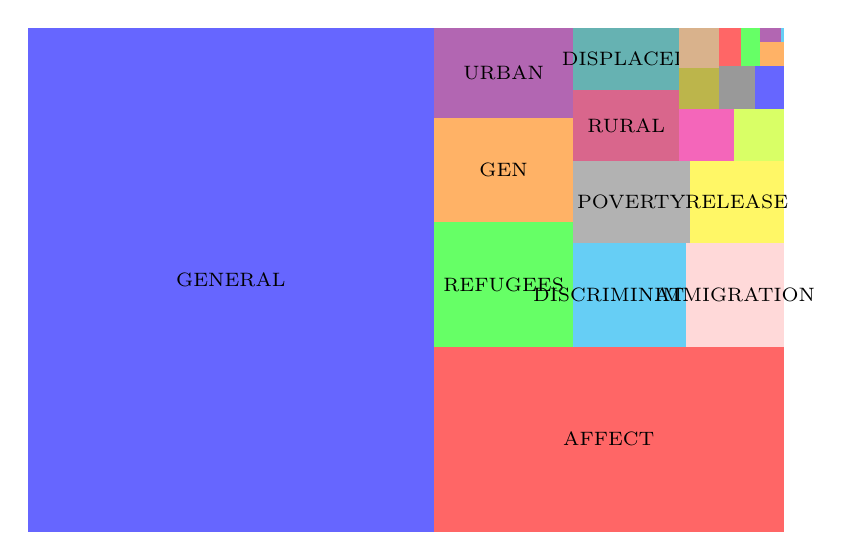
\begin{tikzpicture}[x=0.08cm,y=0.08cm]
% Auto-generated squarified treemap
% Data: 22 items, total value: 5,872,378
\fill[blue!60] (0.00,0.00) rectangle (64.52,80.00);
\node[align=center,font=\scriptsize] at (32.26,40.00) {GENERAL};
\fill[red!60] (64.52,0.00) rectangle (120.00,29.32);
\node[align=center,font=\scriptsize] at (92.26,14.66) {AFFECT};
\fill[green!60] (64.52,29.32) rectangle (86.61,49.12);
\node[align=center,font=\scriptsize] at (75.56,39.22) {REFUGEES};
\fill[orange!60] (64.52,49.12) rectangle (86.61,65.61);
\node[align=center,font=\scriptsize] at (75.56,57.36) {GEN};
\fill[violet!60] (64.52,65.61) rectangle (86.61,80.00);
\node[align=center,font=\scriptsize] at (75.56,72.80) {URBAN};
\fill[cyan!60] (86.61,29.32) rectangle (104.46,45.86);
\node[align=center,font=\scriptsize] at (95.53,37.59) {DISCRIMINATION};
\fill[pink!60] (104.46,29.32) rectangle (120.00,45.86);
\node[align=center,font=\scriptsize] at (112.23,37.59) {IMMIGRATION};
\fill[gray!60] (86.61,45.86) rectangle (105.10,58.76);
\node[align=center,font=\scriptsize] at (95.86,52.31) {POVERTY};
\fill[yellow!60] (105.10,45.86) rectangle (120.00,58.76);
\node[align=center,font=\scriptsize] at (112.55,52.31) {RELEASE};
\fill[purple!60] (86.61,58.76) rectangle (103.43,70.11);
\node[align=center,font=\scriptsize] at (95.02,64.43) {RURAL};
\fill[teal!60] (86.61,70.11) rectangle (103.43,80.00);
\node[align=center,font=\scriptsize] at (95.02,75.05) {DISPLACED};
\fill[magenta!60] (103.43,58.76) rectangle (112.09,67.01);
\fill[lime!60] (112.09,58.76) rectangle (120.00,67.01);
\fill[olive!60] (103.43,67.01) rectangle (109.68,73.61);
\fill[brown!60] (103.43,73.61) rectangle (109.68,80.00);
\fill[black!40] (109.68,67.01) rectangle (115.42,73.88);
\fill[blue!60] (115.42,67.01) rectangle (120.00,73.88);
\fill[red!60] (109.68,73.88) rectangle (113.23,80.00);
\fill[green!60] (113.23,73.88) rectangle (116.27,80.00);
\fill[orange!60] (116.27,73.88) rectangle (120.00,77.68);
\fill[violet!60] (116.27,77.68) rectangle (119.61,80.00);
\fill[cyan!60] (119.61,77.68) rectangle (120.00,80.00);
\end{tikzpicture}